\section{Introduction}
\label{sec:introduction}

Retailers record sales, not demand. When a product sells out, the record stops at the stock that was available and the unmet part of demand leaves no trace. A model fitted to such records learns the stocking policy along with customer behavior, and its errors carry into the next order. Fresh retail makes the cost immediate: tomorrow's order trades lost sales against perishable surplus, and a forecast that tracks recorded sales closely can still lead to a poor order if its history was censored~\cite{nahmias1994demand,huh2011adaptive}. For the same reason, a lower forecast error does not by itself show that one ordering policy is better than another. The comparison has to use the same outcome, the same cost ratio, and the same scored rows.

FreshRetailNet-50K~\cite{wang2025freshretailnet,dingdong2025datasetcard} makes this problem measurable because it records an hourly stock-status flag next to hourly sales. We use the flags in a narrow way. A series-day with no flagged stockout between 06:00 and 21:59 is a \emph{donor day}, and its recorded sales over that window serve as an exact proxy for demand, provided the flags are correct. Donor days are not a random sample: well-stocked and slow-moving items qualify more often, and the proxy says nothing about demand on days that were actually censored. Within that limit, donor days support a controlled experiment. Three simulated stockout mechanisms censor the histories of eligible donor days in different ways. Features and forecasts are rebuilt from each censored history, and every forecast is scored against the same uncensored proxy, so a model trained under one mechanism can be evaluated under another on identical target rows.

The evidence comes from three saved executions of one notebook pipeline (Fig.~\ref{fig:lineage}). Two standalone runs cover the development phases on a stratified 5,000-series sample (run~S) and on all 50,000 series (run~P). A third, end-to-end run (run~E) repeats the development phases on its own 5,000-series sample and continues through deep-learning baselines, a censored-inventory baseline, conformal calibration, ordering, a protocol lock, and a single evaluation of the final week. We keep the three runs apart. Runs~S and~E report identical tuning errors, yet they are different executions with different output files, and only run~E feeds the final evaluation.

Our contributions are an evaluation design and the evidence it produces, rather than a new forecasting architecture:
\begin{itemize}
\item a matched donor-proxy protocol that scores forecasts and orders trained on differently censored histories against identical outcomes, with the evaluation protocol locked before any final-week outcome was read;
\item a comparison of nine ordering policies under three cost ratios that reports the scored population and row count of every policy, including a separate panel for the neural policies, which cover only a declared subset of series;
\item the pre-specified paired contrasts and mechanism-transfer gaps with cluster-bootstrap intervals, and a lower bound on q90 misses for real censored histories, where no demand label exists.
\end{itemize}
The code, saved run outputs, and paper sources are available at \repourl.

\begin{figure}[t]
\centering
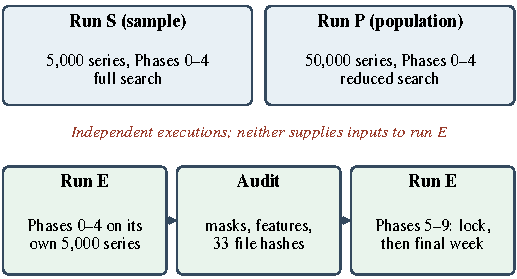
\includegraphics[width=\columnwidth]{figures/run_lineage.pdf}
\caption{The three saved executions. Only run~E's own Phase~0--4 stage feeds its prerequisite audit and the locked final evaluation; runs~S and~P are independent development evidence.}
\label{fig:lineage}
\end{figure}

\subsection{Related work}
\label{sec:related}

Estimating demand from sales truncated by stockouts is a long-standing inventory problem. Parametric methods fit a demand distribution to censored observations~\cite{nahmias1994demand}, and nonparametric policies learn order levels from censored sales with the Kaplan--Meier product-limit estimator~\cite{kaplan1958nonparametric,huh2011adaptive}; our Kaplan--Meier baseline follows the second idea with pooled support rules. Feature-based newsvendor methods learn an order directly from covariates~\cite{ban2019bignewsvendor}. Under linear shortage and surplus costs, the optimal order is a quantile of the demand distribution at the critical fractile, which ties ordering to quantile regression and its pinball loss~\cite{koenker1978regression}.

Our forecasters are gradient-boosted trees~\cite{ke2017lightgbm}, TimesNet~\cite{wu2023timesnet} for recovering masked hours, and the Temporal Fusion Transformer (TFT)~\cite{lim2021tft} for next-day forecasts. Calibration applies pooled split-conformal corrections in the spirit of conformalized quantile regression~\cite{romano2019cqr}, a sequential variant that updates its target miss rate as in adaptive conformal inference~\cite{gibbs2021adaptive}, and monotone rearrangement to remove quantile crossing~\cite{chernozhukov2010quantile}. The coverage guarantees of these methods rest on exchangeability or on explicit assumptions about how the data change; real stockout-censored days meet neither, so we measure coverage only where the donor proxy exists. Intervals come from a percentile cluster bootstrap~\cite{efron1979bootstrap}. The dataset report~\cite{wang2025freshretailnet} introduces the stockout annotations and a two-stage recovery-then-forecast baseline, whose official code~\cite{dingdong2025baseline} we reproduced only in part (Section~\ref{sec:deepdev}).
